%%%%%%%% this is our results and comparison

%\documentclass[12pt, amstex, letterpaper] {report} %{article}


\usepackage[margin=1in]{geometry}
\topmargin -0.5in \textwidth 6.5in \textheight 9in
\footskip .5in
\headheight 0.3in


\usepackage{Sweave}

\DefineVerbatimEnvironment{Sinput}{Verbatim} {xleftmargin=0em,frame=single}
\DefineVerbatimEnvironment{Soutput}{Verbatim} {xleftmargin=0em,frame=single}

\usepackage{amssymb, mathrsfs, amsmath, amsfonts}
\usepackage{enumerate, comment}
\usepackage{hyperref, natbib,apalike, float} %cite
\usepackage{color, multirow, setspace, fancyhdr,graphicx}
\usepackage{undertilde}
\usepackage[bottom]{footmisc}
\usepackage{graphicx}
\usepackage{framed}
\usepackage{subcaption}
\usepackage{amsthm}

%\doublespacing
\pagestyle{empty}
\pagestyle{fancy}
\lhead{ }
%\rhead{May 2016}
\fancyfoot{ }
\rfoot{Dissertation $|$ \thepage}
\lfoot{Chris Vanlangenberg}
\date{}

\includecomment{comment}

\newtheorem{theorem}{Theorem}[section]
\newtheorem{defn}{Definition}[section]
\newtheorem{prop}{Proposition}
\newcommand{\pro}[1]{\begin{prop}{#1}\end{prop}}

%\newtheorem{proof}{proof}
\newtheorem{rmk}{Remark}
\newcommand{\rmark}[1]{\begin{rmk}{#1}\end{rmk}}

\numberwithin{equation}{section}
\renewcommand{\footrulewidth}{0.1pt}
\renewcommand{\headrulewidth}{0.1pt}


\newcommand{\eqn}[1]{\begin{equation}{#1}\end{equation}}

\newcommand{\beq}{\begin{equation}}
\newcommand{\eeq}{\end{equation}}
%\renewcommand\refname{Literature}
\newcommand{\blue}[1]{\textcolor{blue}{\emph{#1}}}
\newcommand{\red}[1]{\textcolor{red}{\emph{#1}}}
\newcommand{\twoc}[2]{{\textcolor{blue}{#1}} and {\textcolor{red}{#2}}}


\newcommand{\xn}{x_1,\ldots, x_n}
\newcommand{\Xn}{X_1,\ldots, X_n}
\newcommand\floor[1]{\lfloor{#1}\rfloor}
\newcommand\ceil[1]{\lceil{#1}\rceil}

\newcommand{\X}{\mathcal{X}}
\newcommand{\Sp}{\mathbb{S}}
\newcommand{\R}{\mathbb{R}}
\newcommand{\C}{\mathbb{C}}
\newcommand{\pd}{positive definite }



\newcommand{\code}[1]{{\small\texttt{#1}}}
\newcommand{\pkg}[1]{{\normalfont\textsf{#1}}}
\newcommand{\var}[1] {{\normalfont\textbf{#1}}}
\newcommand{\Cm}{$C_m(\phi_P, \phi_Q)\ $}

\newcommand{\jun}{\cite{JunStein2008}}
%\begin{document}

To our knowledge, currently there are no methods developed to test axially symmetry in global data, in fact this could be another research opportunity in spatial statistics. Therefore, to validate the compatibility of generated axially symmetric global data we compared the MOM estimate to its theoretical value more preciously the cross variogram estimator. The cross variogram estimator (\ref{cross_variogram}) is unbiased and in the case of circle we showed that variogram estimator is inconsistent and we expect a similar result in the case of sphere (the proof is left out as future work). We consider multiple to compare the simulated data at multiple pairs of latitudes with fixed number of longitudes ($n_L = 100$). The cross variogram estimator is almost identical to it's theoretical value if pairs (latitudes) were closer. Therefore we will demonstrate a case with larger latitude difference ($\phi_P = 10^0, \phi_Q = 150^0$ equivalent to $70^0S$ and $60^0N$) in which will capture the largest possible errors.

%The rate of convergence (\blue{should we talk about any theoretical properties of convergence since we don't have a proof for consistency}) is very slow as one can see that when number of simulations were increased from 500 to 4000 the cross variogram estimator is much closer to its theoretical value. However, the cross variogram estimator for model 2 and 3 converges much faster compared to model 1. 

\vskip 24pt

%-------------------------------------% 
\subsection{\bf Comparison of MOM estimators}
%-------------------------------------%

Now we compare the cross variogram estimator given in $\eqref{cross_variogram}$, when using $R(P,Q)$ directly compared to proposed $C_m$ approach. Higher dimension is the biggest draw back when using $R(P,Q)$ directly and in some occasions $R(P,Q)$ will provide negative eigen values for example model 3. Hence one cannot perform SVD to generate data. In contrast, it is guaranteed that \Cm is positive definite and Hermitian. However, it might be a challenge to derive \Cm from a given $R(P,Q)$ model.    

\begin{figure}[H]
	\begin{subfigure}{.5\textwidth}
		\centering
		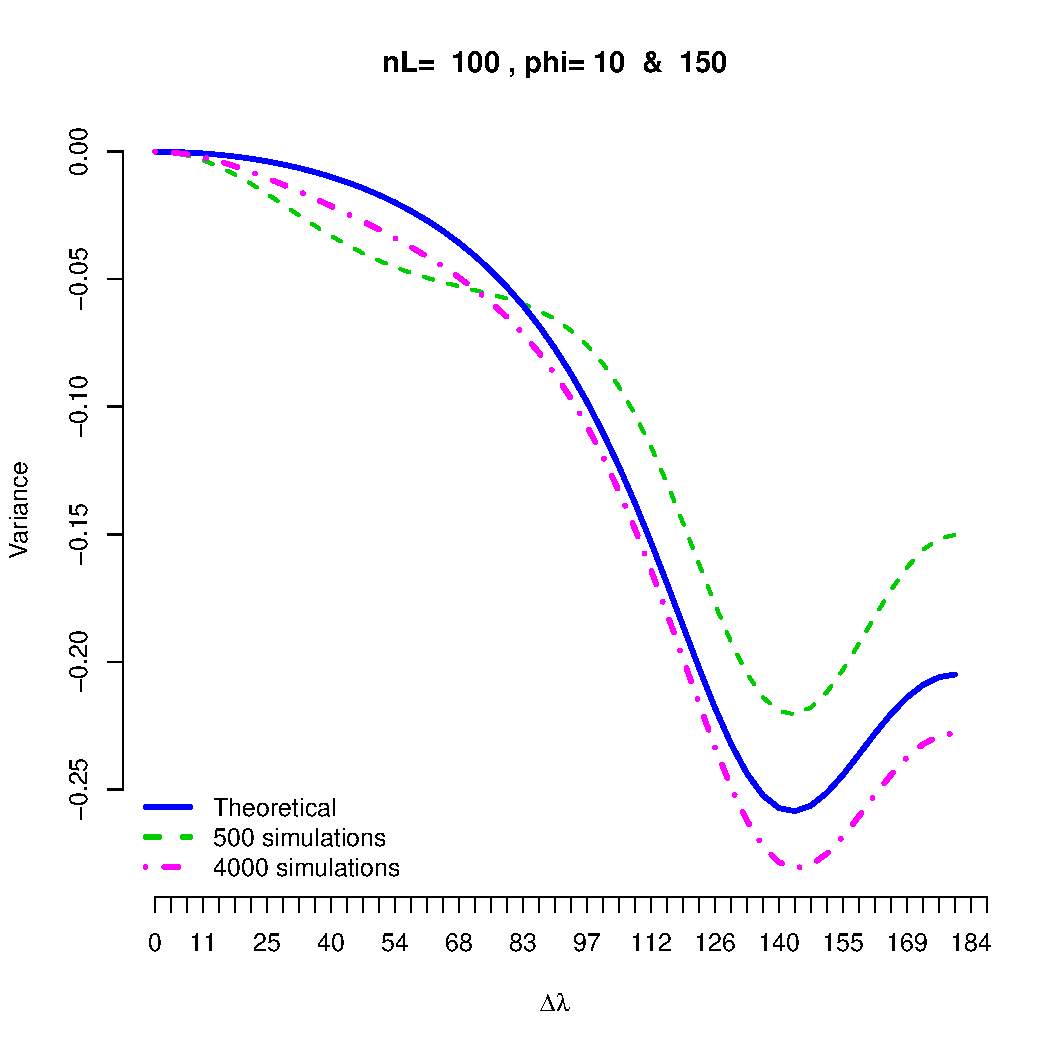
\includegraphics[width=1\linewidth]{graphs/results_variogram_model1_rpq}
		\caption{Using paramter Set 1 and $R(P,Q)$}
		\label{fig:sfig1}
	\end{subfigure}
	\begin{subfigure}{.5\textwidth}
		\centering
		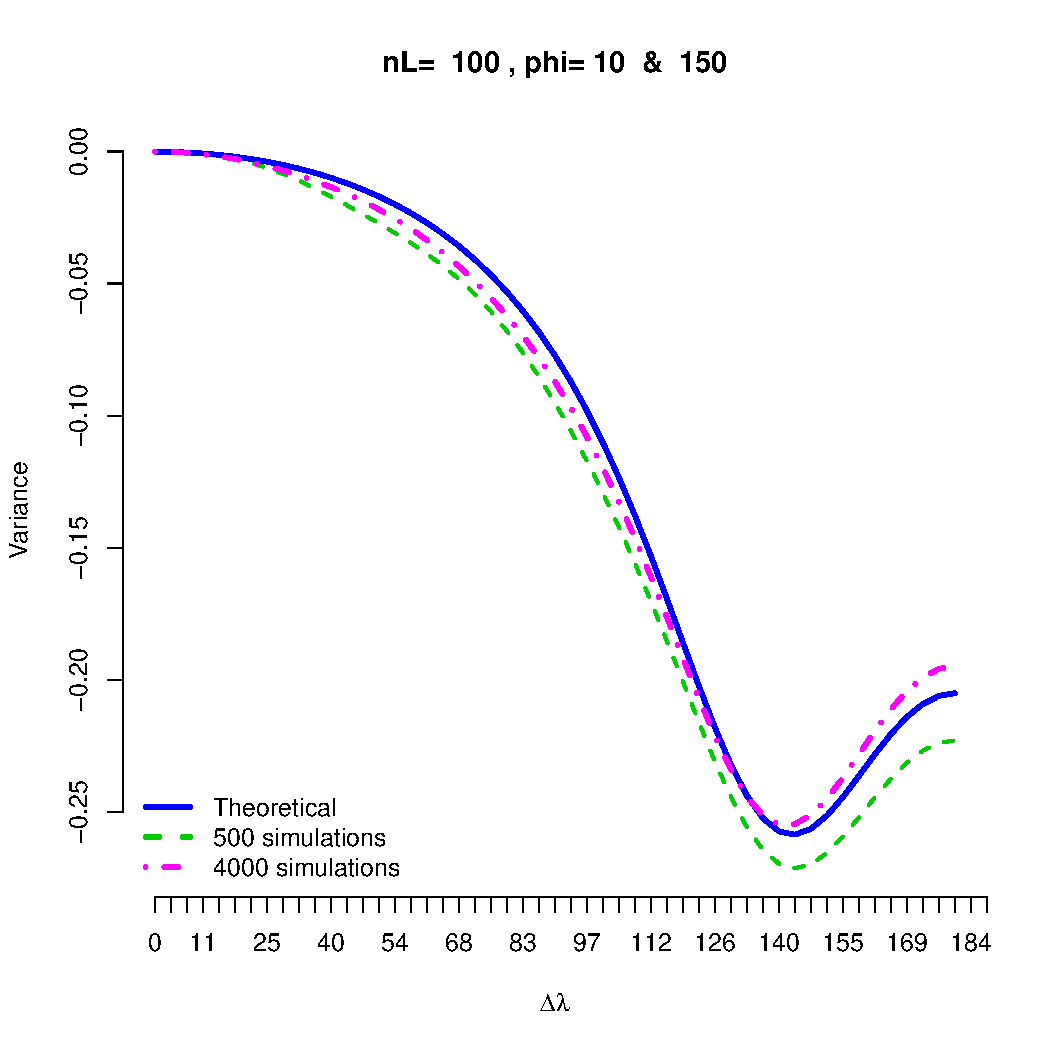
\includegraphics[width=1\linewidth]{graphs/results_variogram_model1}
		\caption{Using paramter Set 1 and $C_m$}
		\label{fig:sfig2}
	\end{subfigure}
	\begin{subfigure}{.5\textwidth}
		\centering
		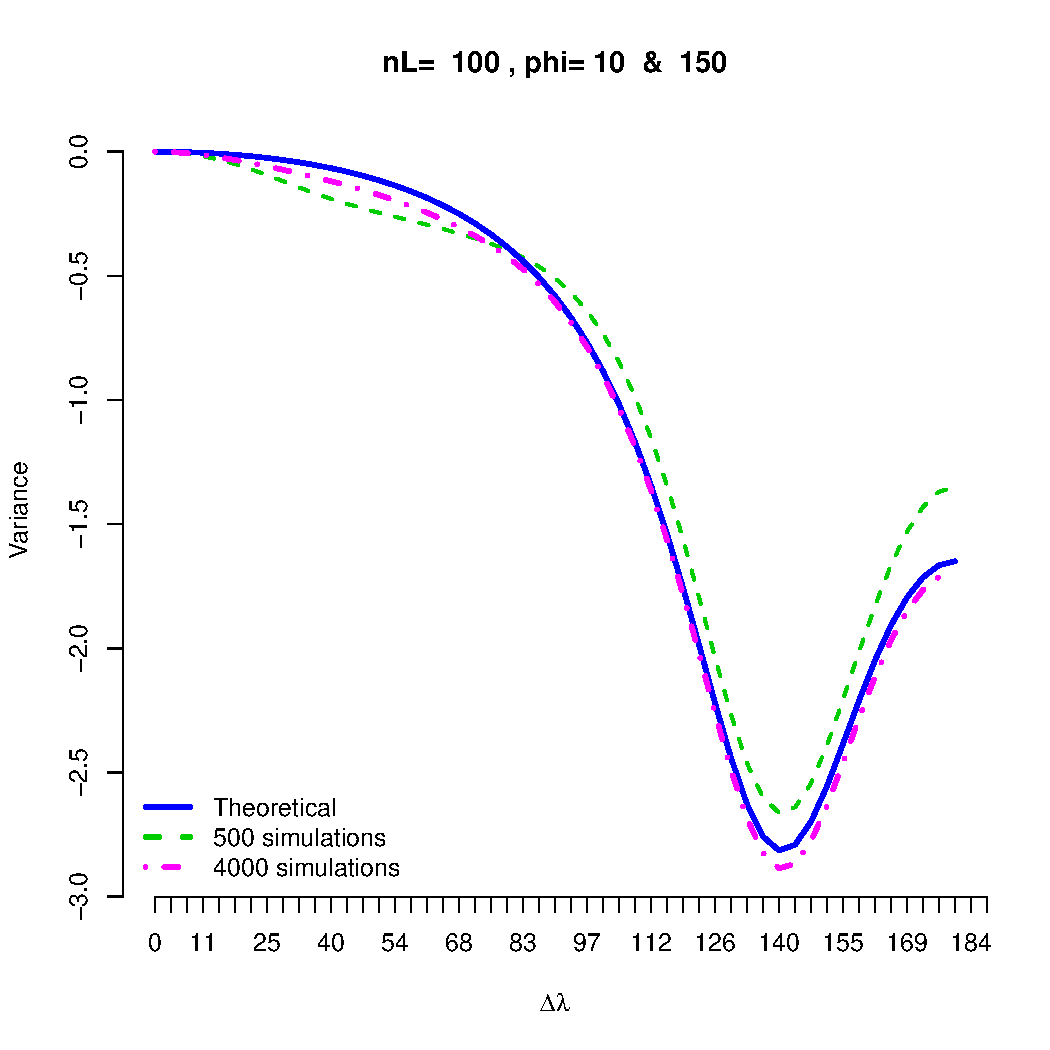
\includegraphics[width=1\linewidth]{graphs/results_variogram_model1_rpq_2}
		\caption{Using paramter Set 2 and $R(P,Q)$}
		\label{fig:sfig1}
	\end{subfigure}
	\begin{subfigure}{.5\textwidth}
		\centering
		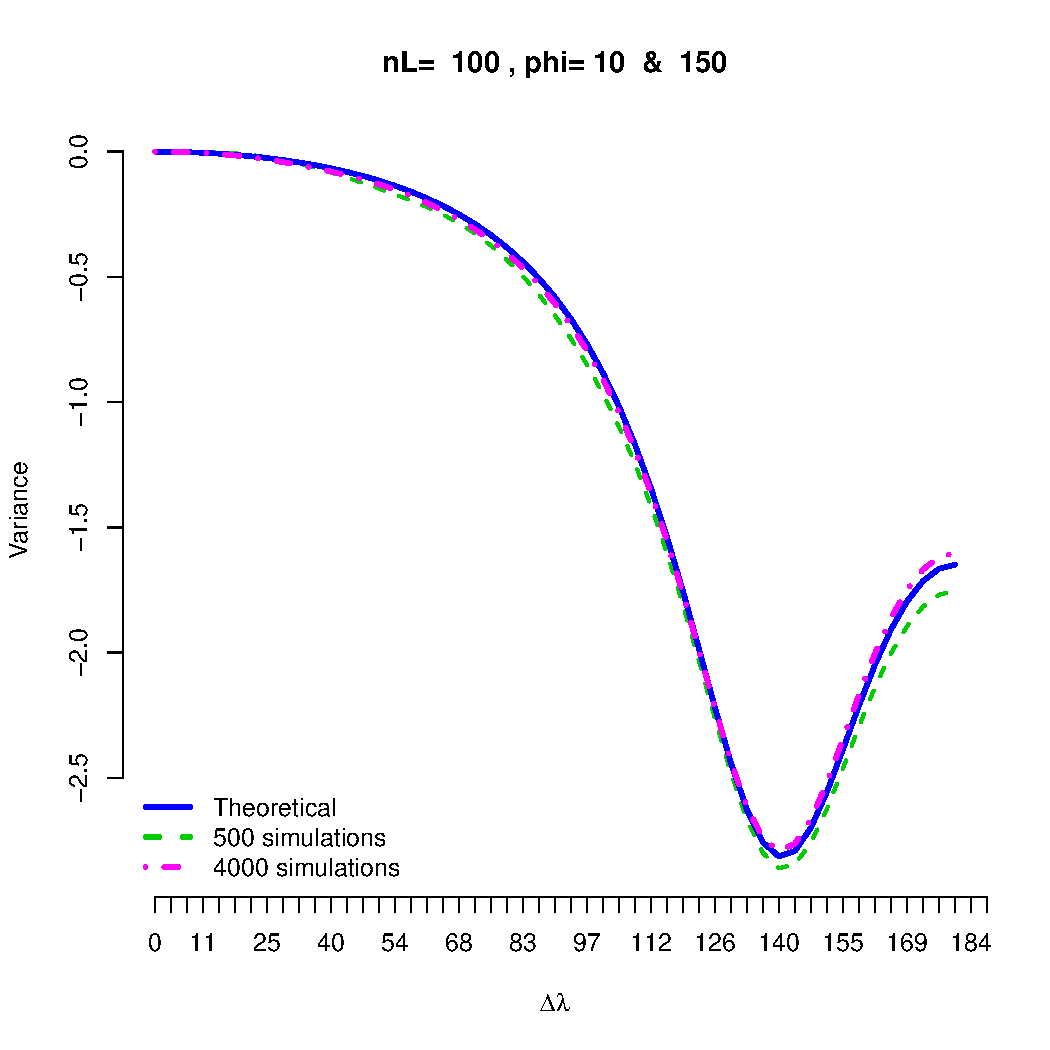
\includegraphics[width=1\linewidth]{graphs/results_variogram_model1_2}
		\caption{Using paramter Set 2 and $C_m$}
		\label{fig:sfig2}
	\end{subfigure}
	\caption[Cross variogram estimator comparison]{Using parameter Set 1 and Set 2 to compare variogram estimator for model 1, solid line (blue) the theoretical values of cross variogram and dashed lines (green, purple) represents the estimates for 500 and 4000 simulations respectively. }
	\label{compare_varigram_sim_1}
\end{figure}


% 
% \begin{figure}[H]
% 	\begin{subfigure}{.5\textwidth}
% 		\centering
% 		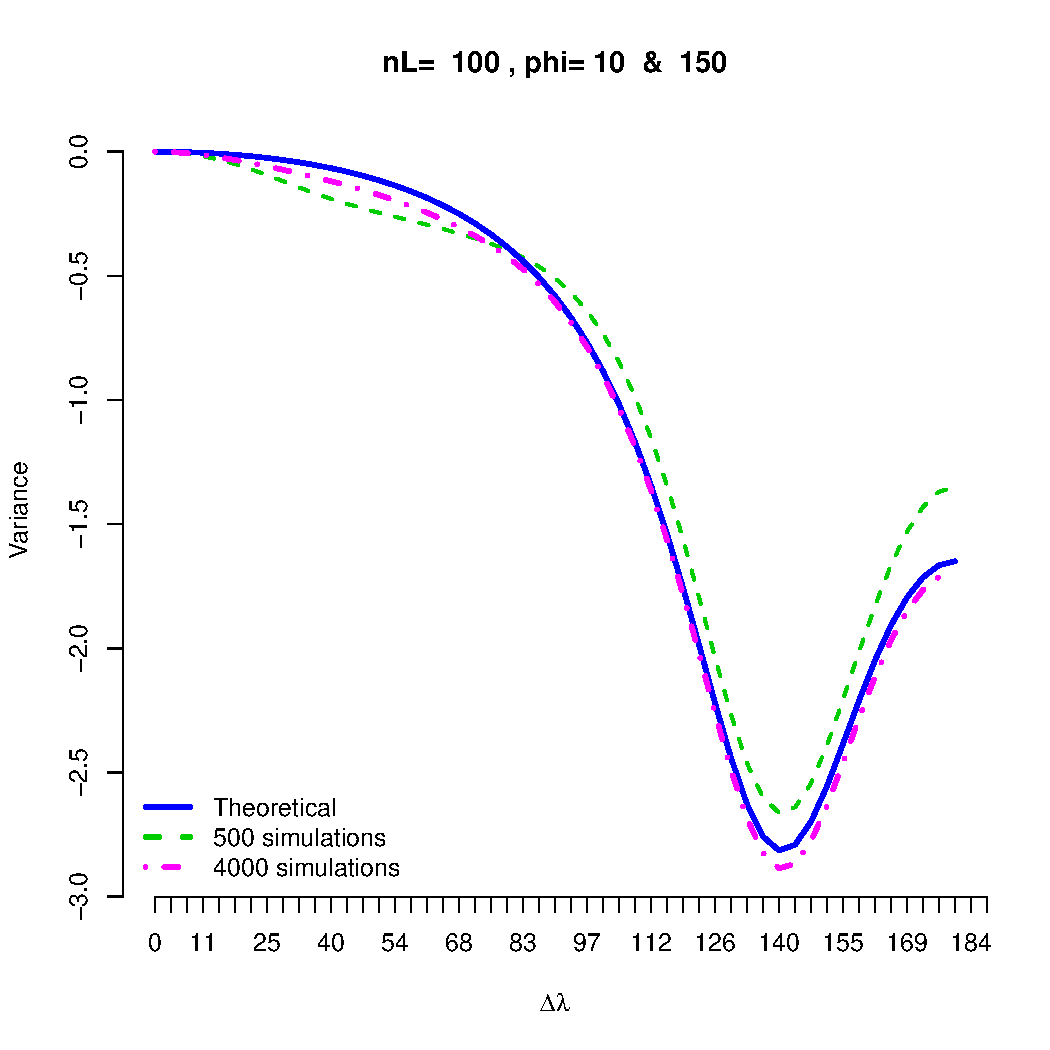
\includegraphics[width=1\linewidth]{graphs/results_variogram_model1_rpq_2}
% 		\caption{Using $R(P,Q)$}
% 		\label{fig:sfig1}
% 	\end{subfigure}
% 	\begin{subfigure}{.5\textwidth}
% 		\centering
% 		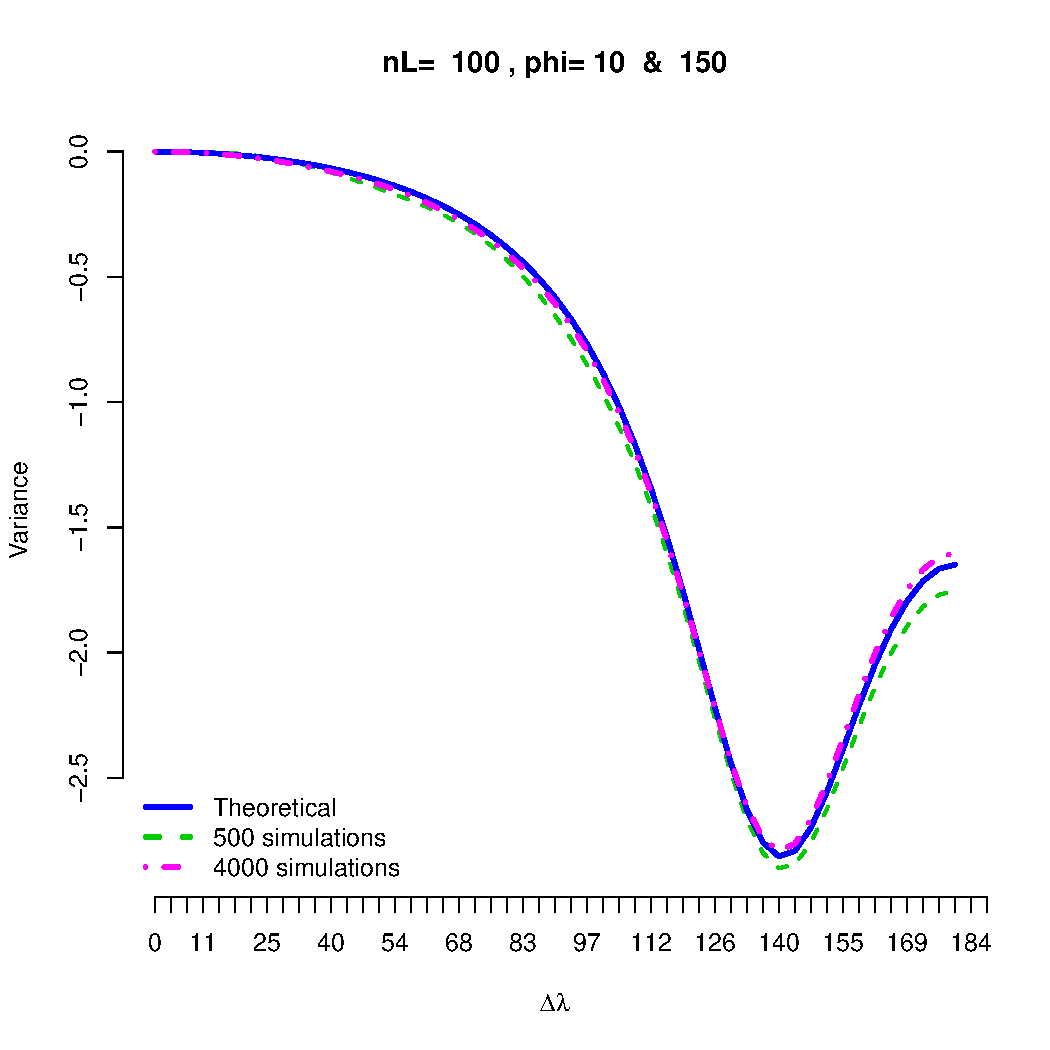
\includegraphics[width=1\linewidth]{graphs/results_variogram_model1_2}
% 		\caption{Using $C_m$}
% 		\label{fig:sfig2}
% 	\end{subfigure}
% 	\caption[Cross variogram estimator comparison]{Cross variogram comparison using parameter set 2 similar to \ref{compare_varigram_sim_1}}
% 	\label{compare_varigram_sim_2}
% \end{figure}



%-------------------------------------% 
\subsection{\bf Results for longitudinally reversible processes}
%-------------------------------------%

The parameter $u = 0$ yields a longitudinally reversible processes on a sphere (see Figure \ref{fig_parameter_comp} 1(d) ) in all proposed models. In all three models the cross variogram estimator converges ({\em a.s.}) to its theoretical value (< 500 simulations).          

\begin{figure}[H]
	\centering
	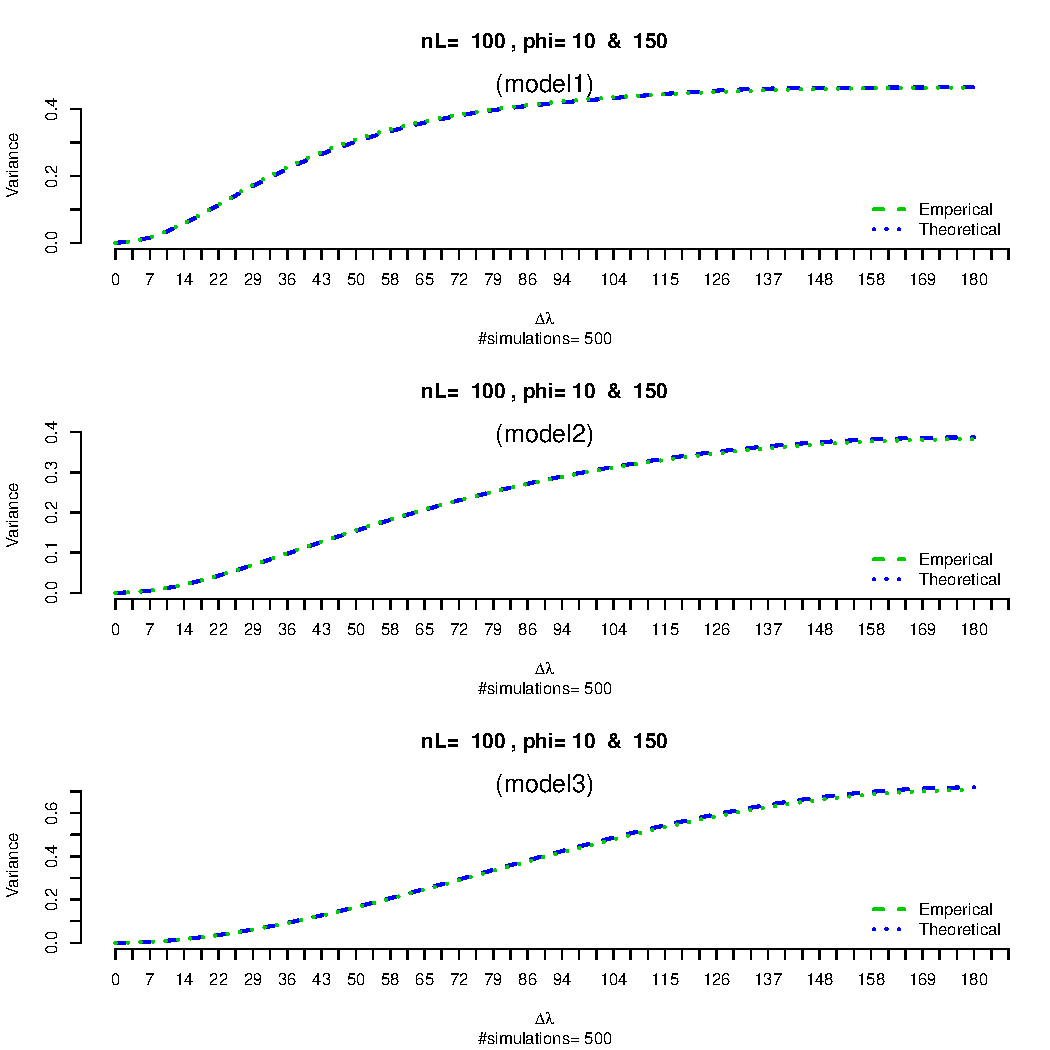
\includegraphics [width=0.9\textwidth ]{graphs/results_variogram_comparison}
	% width=12cm,height=12cm
	\caption[Variogram comparison]{The cross variogram estimator comparison for longitudinally reversible process using  model 1, model 2 and model 3 (when $u=0$).}
\end{figure}

%-------------------------------------%
\subsection{\bf Comparison of cross covarince}
%-------------------------------------%

When the random process on a sphere is non zero mean, the cross covariance estimator is biased ($c_0 \ne 0$). Therefore we compared the cross covariance estimator given by \ref{cross_covariance} for zero mean processes (model 2, model 3) on a sphere. In order to compare the cross covariance we used two pairs of latitudes, $\phi = 70, 80$ ($20^0S$ ,$10^0S$) and $\phi = 60, 120$ ($30^0S$, $40^0N$). The cross covariance estimate match with the theoretical value   

% \begin{figure}[H]
% \begin{center}
% 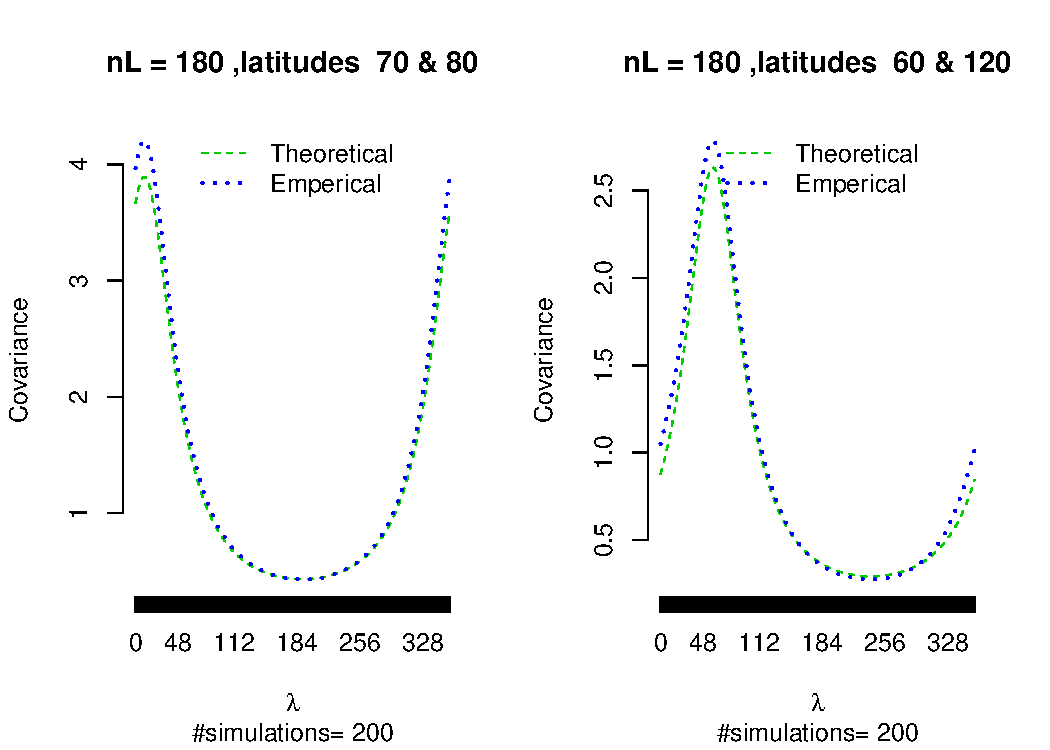
\includegraphics [width=0.75\textwidth ]{graphs/Model1.pdf}
% \caption{Cross covariance comparison of model1}
% \end{center}
% \end{figure}

% \begin{columns}
% \begin{figure}[H]
% 
% \column{\textwidth}
% 	\begin{cen}
% 		\includegraphics [width=0.75\textwidth ]{graphs/Model2.pdf}
% 		%\includegraphics [width=6in, height=3in]{Model2.pdf}
% 		%\caption{Cross covariance comparison of model 2}
% 	\end{center}
% %\end{figure}
% \column{\textwidth}
% %\begin{figure}[H]
% 	\begin{center}
% 		%\includegraphics [scale=.6]{Model3.pdf}
% 		\includegraphics [width=0.75\textwidth ]{graphs/Model3.pdf}
% 		\caption{Cross covariance comparison of model 3}
% 	\end{center}
% \end{figure}
% \end{columns}
% 
% \begin{columns}
% \begin{figure}[H]

\begin{figure}
	\begin{subfigure}{1\textwidth}
		\centering
		\includegraphics[keepaspectratio, scale=0.8]{graphs/Model2}
		\caption{Model 2 \eqref{model2}}
		\label{fig:cov2}
	\end{subfigure}
	\begin{subfigure}{1\textwidth}
		\centering
		\includegraphics[keepaspectratio, scale=0.8]{graphs/Model3}
		% \includegraphics[width=1\linewidth]{graphs/Model3}
		\caption{Model 3 \eqref{model3}}
		\label{fig:cov3}
	\end{subfigure}
\caption{Cross covariance comparison of model 2 and model 3}
\end{figure}


The proposed covariance models are functions of latitude difference and the cross covariance estimator converges to its theoretical value with fewer simulations when the difference is small compared to larger latitude differences (the slow convergence at inflection points).     

\vskip 24pt

%-------------------------------------%
\subsection{\bf Comparison of MSE}
%-------------------------------------%

The mean square error (MSE) of cross variogram was computed for both $C_m$ and direct $R(P,Q)$ approaches. In order to compute the MSE multiple pairs of latitudes where considered,

\begin{eqnarray*}
MSE &=& \frac{1}{n_L} \sum (var + bias^2) \\
    &= & \frac{1}{n_L} \sum_{j=1}^{n_L} \left[ \frac{1}{nn}\sum_{i=1}^{nn}\left(\hat{\gamma_{i}}(j\Delta\lambda)-\overline{\hat{\gamma}(j\Delta\lambda)})^2\right) +  (\gamma_(j\Delta\lambda) - \overline{\hat{\gamma}(j\Delta\lambda)})^2 \right]
\end{eqnarray*}

\begin{table}[H]
\label{parameters}
\centering
\begin{tabular}{|l|c|l|l|l|l|}
\hline 
\multicolumn{2}{|c|}{}  & \multicolumn{2}{|c|}{Set 1} & \multicolumn{2}{|c|}{Set 2}  \\ \hline
  Model                 & $(\phi_P, \phi_Q)$    & $R(P,Q)$  & $C_m$  & $R(P,Q)$  & $C_m$  \\ \hline
\multirow{3}{*}{Model1} & (60, 90)  & 2.300     & 2.427	& --	& --	 \\
                        & (50, 100) & 1.784     & 1.782	& --	& --	 \\ 
                        & (10, 150) & 0.564     & 0.623	& --	& --	 \\ \hline
\multirow{3}{*}{Model2} & (60, 90)  & 2.000     & 2.080	& 12.452	& 13.021 \\  
                        & (50, 100) & 1.437     & 1.459	& 9.196	  & 9.262 \\  
                        & (10, 150) & 0.457     & 0.512	& 6.034	  & 7.266 \\ \hline 
\end{tabular}
\caption{MSE comparison for $C_m$ and $R(P,Q)$ approaches, Set 1 and Set 2 are referring to the set of parameters discussed in simulation setup}
\end{table}


\begin{figure}[H]
	\begin{subfigure}{.5\textwidth}
		\centering
		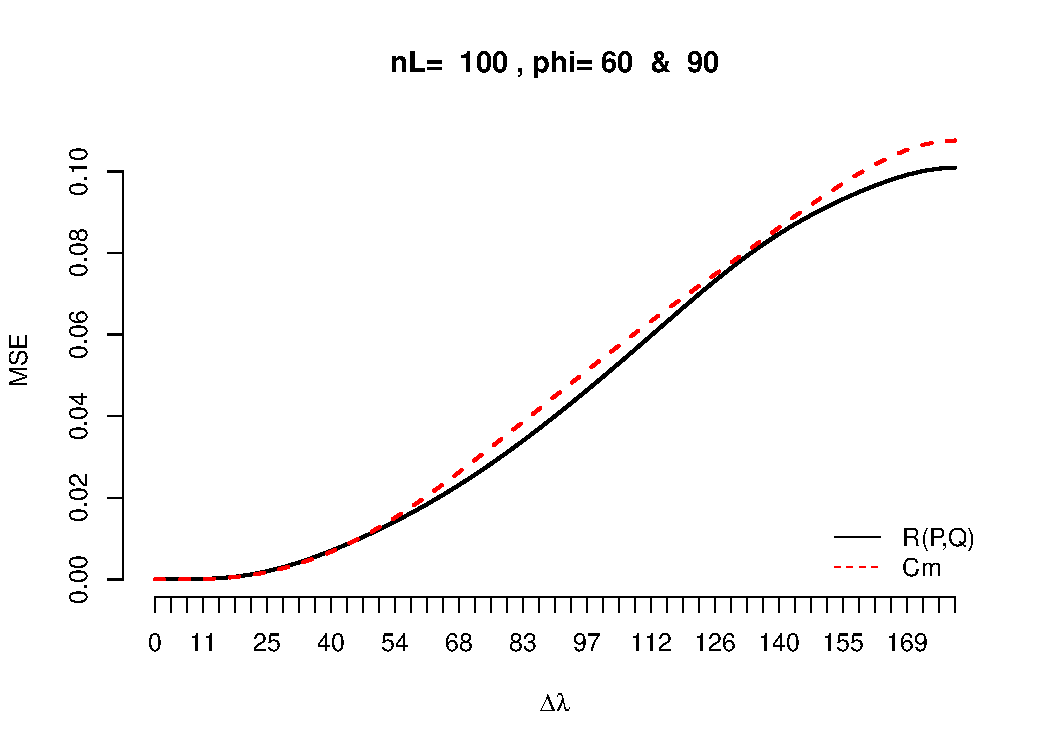
\includegraphics[width=1\linewidth]{graphs/MSE_comparison_model1_60_90}
		\caption{Model 1 (pair 1)}
		\label{fig:mse1}
	\end{subfigure}
	\begin{subfigure}{.5\textwidth}
		\centering
		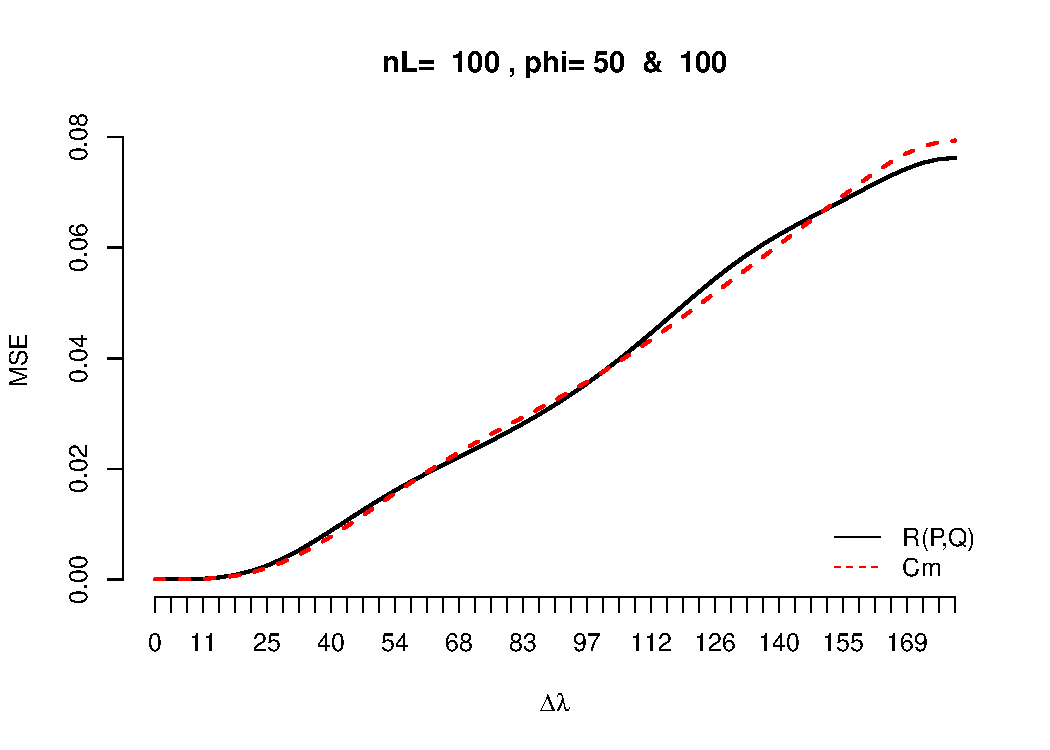
\includegraphics[width=1\linewidth]{graphs/MSE_comparison_model1_50_100}
		\caption{Model 1 (pair 2)}
		\label{fig:mse2}
	\end{subfigure}
		\begin{subfigure}{.5\textwidth}
		\centering
		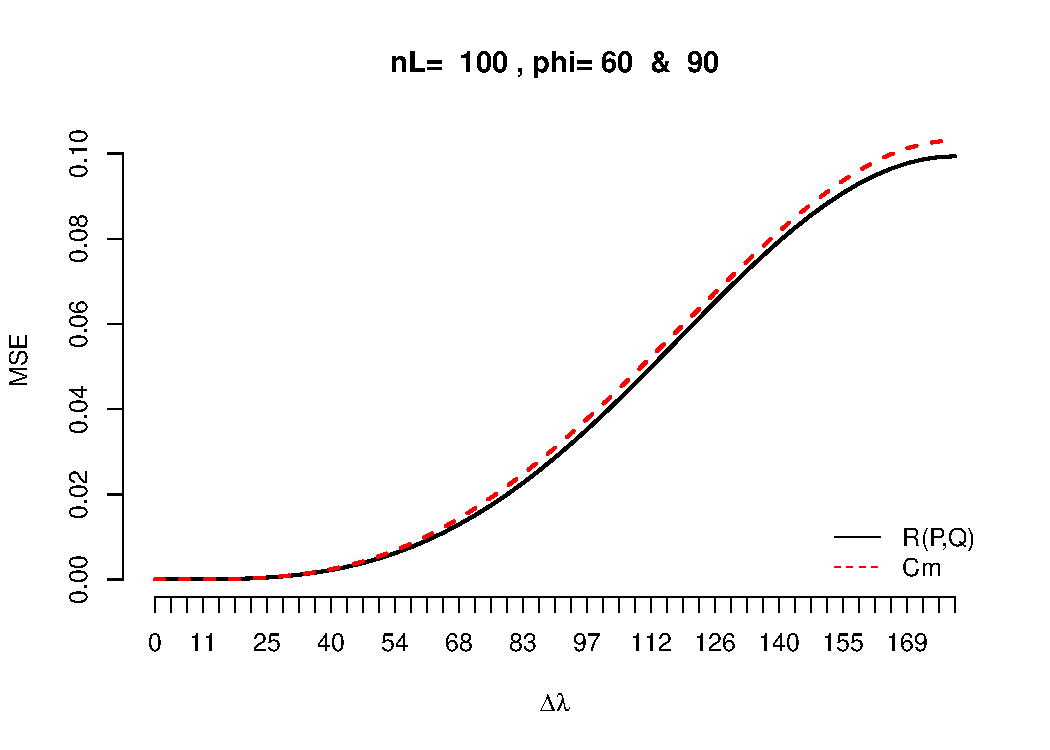
\includegraphics[width=1\linewidth]{graphs/MSE_comparison_model2_60_90}
		\caption{Model 2 (pair 1)}
		\label{fig:mse3}
	\end{subfigure}
		\begin{subfigure}{.5\textwidth}
		\centering
		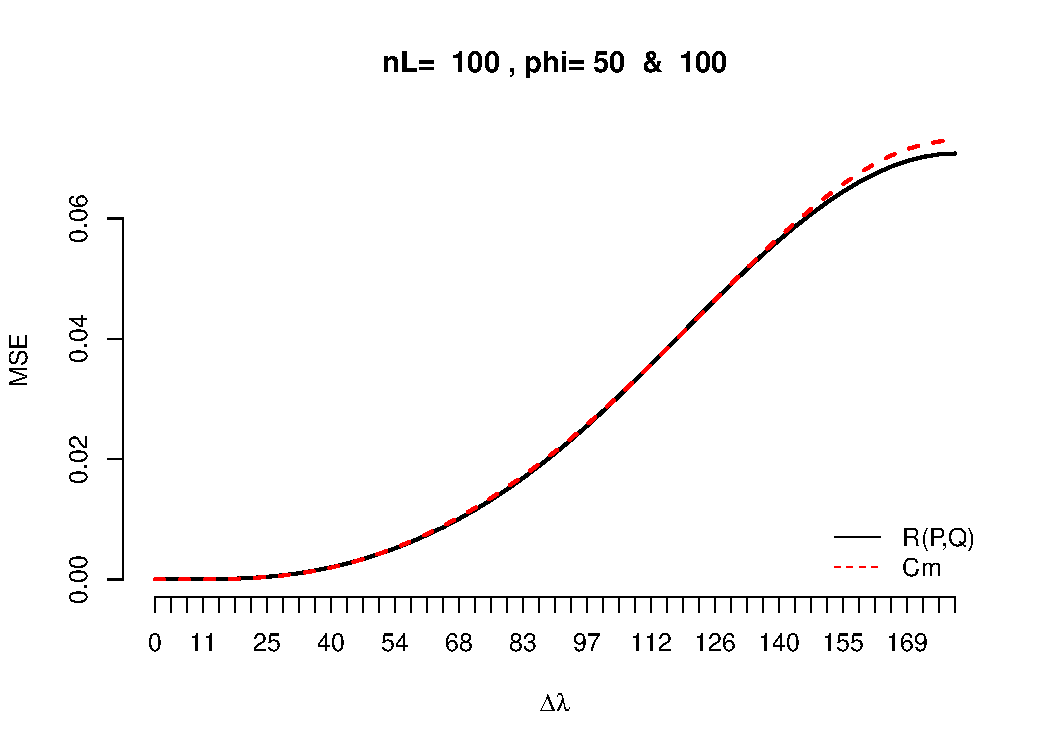
\includegraphics[width=1\linewidth]{graphs/MSE_comparison_model2_50_100}
		\caption{Model 2 (pair 2) }
		\label{fig:mes4}
	\end{subfigure}
	\caption[]{MSE comparison between $C_m$ and $R(P,Q)$ using 500 simulations; pair 1 ($30^0S,0^0$), pair 2 ($40^0S, 10^0N$) figures (a) - (b) is the comparison for model 1 and figure (c)-(d) is the comparison for model 2 }
	\label{mse_comparison}
\end{figure}

Based on 500 simulations the MSE for $C_m$ is closer to its counter part, $R(P,Q)$. However, one should consider the huge reduction in dimension when using the proposed $C_m$ approach. In the data generation process it is not computationaly feasible to perform a SVD with large dimensions.  Moreover, obtaining $R(P,Q)^{1/2}$ with the light of block circulant matrix properties seems unclear as we cannot obtain real-valued eigen values for proposed model 3 \eqref{model3}. In our approach MSE slightly higher (almost similar) higher, high variance but low bias compared to direct R(P, Q).  

% 
% \[
% MSE = \frac{1}{n_L-1}\sum_{k=1}^{n_L} (\gamma_{k}(\Delta\lambda) - \overline{\hat{\gamma}_{k}(\Delta\lambda)})^2
% \]

% \begin{table}[H]
% \label{parameters}
% \centering
% \begin{tabular}{|l|l|l|l|l|l|l|}
% \hline 
%  & \multicolumn{2}{|c|}{Model 1} & \multicolumn{2}{|c|}{Model 2} & \multicolumn{2}{|c|}{Model 3} \\ \cline{2-7}
% Parameters & $R(P,Q)$  & $C_m$  & $R(P,Q)$  & $C_m$ & $R(P,Q)$  & $C_m$ \\ \hline 
% % set 1 & 	0.04825 & 0.00881   & 	0.01820 & 0.00534 & 	-- & 0.01426 \\
% % set 2 & 	1.15598 & 0.16591   & 	0.42931 & 0.14270 & 	-- & 0.33726 \\ \hline \hline
% 
% set 1 & 0.000965 &  0.0001762	& 0.000364	& 0.000107	&--&	0.0002852 \\
% set 2 & 0.023119 &  0.0033182	& 0.0085862	& 0.002854	&--&	0.0067452 \\ \hline \hline 
% 
% %model 1 4000 Cm 0.03085625
% %model 1 4000 R(P,Q) 0.1144611
% 
% \end{tabular}
% \caption{MSE comparison}
% \end{table}

% Now the MSE for $R(P,Q)$ is lower but the bias is higer (bias for $C_m = 0.0325219$ and $R(P,Q) = 0.2493109$.)


%-------------------------------------% 
\subsection{\bf Generated data}
%-------------------------------------%

\begin{figure}[H]
	\centering
		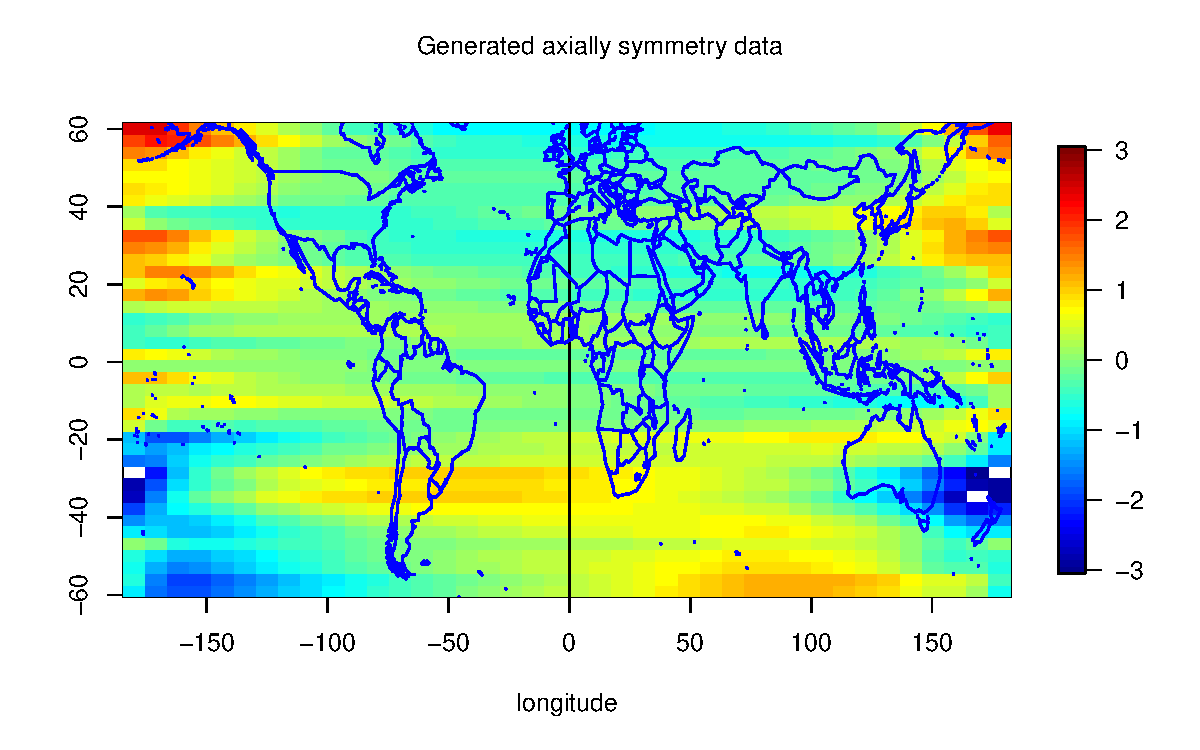
\includegraphics [width=1\textwidth ]{graphs/Data_sample_120_model2_withmap.pdf}
		\caption[A snapshot of global data generated based]{A snapshot of global data generated based on $C_m$ approach using zero mean random process (model 2)}
		\label{grid_plot_model_2}
\end{figure}

The above figure is a snapshot of the global data generated based on model 2 and are some what compliance with practical geo-spatial data (MSU and TOMS), clearly there are spatial trends within the latitudes but not within longitudes. However we observed some inconsistencies (strong spots) closer to the boundary points of longitudes ($\lambda \rightarrow \pm\pi$). 

\begin{figure}[H]
	\label{grid_plot_model2_sim2}
	\begin{center}
		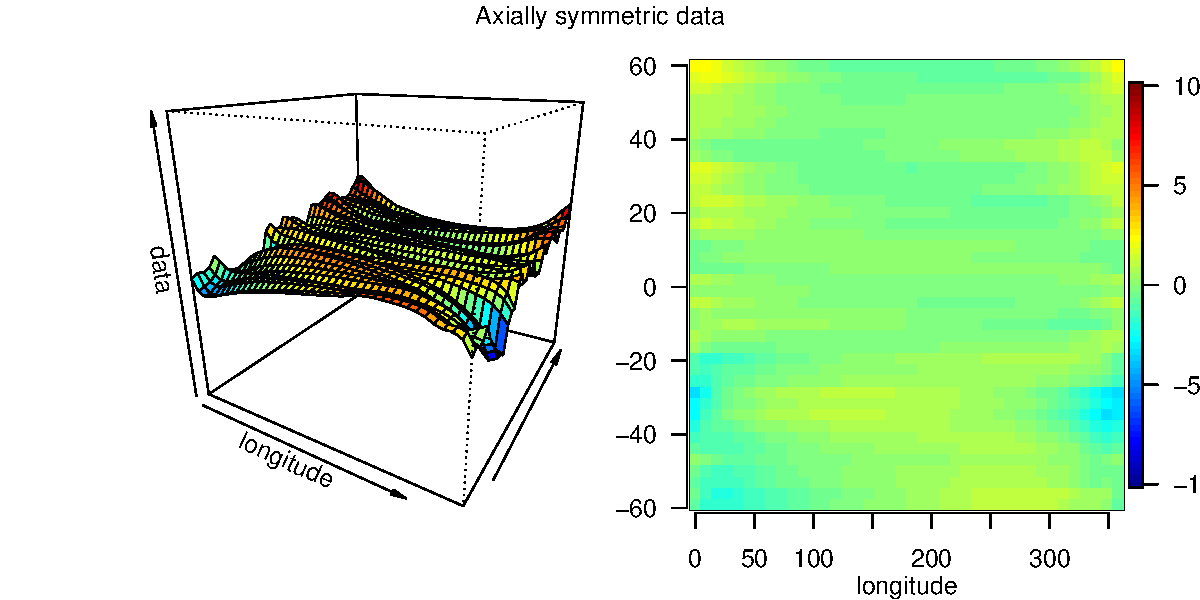
\includegraphics [width=0.9\textwidth ]{graphs/Data_sample_120_model2_density.pdf}
		\caption{One snapshot of the axially symmetric data generated based on model 2, grid resolution $2^0\times 1^0$ (data scale -10 and 10).}
	\end{center}
\end{figure}

The above figure refers to the data snapshot given by figure \eqref{grid_plot_model_2} and it is clearly evident that trends are within latitudes not within longitudes. Four snapshots of the gridded data generated based on all models are given in appendix \ref{appendixA}.

%\end{document}
